\documentclass[a4paper]{article}
\usepackage{ulem}
\usepackage{setspace}
\usepackage{wrapfig}
\usepackage{bpchem}
\usepackage{color}
\usepackage{subfigure}
\usepackage{float}
\usepackage{titletoc}
\usepackage{indentfirst}
\usepackage{geometry}
\usepackage{amsmath}
\usepackage{amssymb}
\usepackage{graphicx}
\usepackage{enumerate}
\usepackage{url}
\usepackage{caption2}
\usepackage{graphicx}  
\usepackage{epstopdf}
\usepackage{listings}
\lstloadlanguages{[5.2]Mathematica}

\geometry{a4paper,left=2.54cm,right=2.54cm,top=2.54cm,bottom=2.54cm}

\begin {document}
\begin{large}
	\begin{center}
	~\\ ~\\ ~\\ ~\\ ~\\ ~\\ \rule[-1pt]{10.3cm}{0.05em} \\~\\UM-SJTU JOINT INSTITUTE\\~\\Probabilistic Methods in
Engineering\\~\\(VE401)	~\\ \rule[-1pt]{10.3cm}{0.05em} \vspace{7cm} \\Term Project 2
	\end{center}
\end{large}
~\\

\begin{large}
	\begin{center}
	Police Shootings in the United States
	\end{center}
\end{large}
\vspace{5cm}

\begin{tabular}{l l l}
	Name: Feitong Tang&ID: 518370910017&Group 1\\
	Name: Weikai Zhou&ID: 518021911039&Group 1\\
     ~\\
	Date: 30 April 2020
\end{tabular}

\newpage

\section{Abstract}
	Based on David Spiegelhalter and Arthur Barnett's \textit{London murders: a predictable pattern?}, this project analyzes the pattern of occurrence of fatal police shootings in the United States. The project gets its data from the database of the Washington Post and gives an overview of the data. It uses goodness-of-fit test to check whether the occurrence of fatal police shooting in the United States follows a Poisson distribution in the years 2015-2019. It also tests whether the average number of police shootings depends on weekdays. It gives the confidence interval for the parameter $k$ of a Poisson distribution. Based on the data from Jan. 1 to Apr. 15, 2020, it tests whether it follows a Poisson distribution and calculates $\hat{k}_{2020}$. It gives the 95\% prediction intervals for the number of police shootings in 2020 and analyzes how COVID-19 will influence the data for 2020.
\\

\noindent\textbf{Keywords}: Fatal police shooting in the United States, Poisson distribution, goodness-of-fit test, confidence interval, prediction interval.



\newpage

\tableofcontents

\newpage

\section{Introduction}
	\subsection{Background}
	David Spiegelhalter and Arthur Barnett analyzed the pattern of London murders between April 2004 and March 2007, and predicted the number of murders in London during 2008 [1]. Based on their analysis and the data of fatal police shootings in the USA provided by Washington Post [2], we want to analyze the pattern of fatal police shootings in the USA from January 2015, and predict the number of fatal police shootings in 2020.

	\subsection{Objectives}
	\begin{itemize}
	\item Give an overview of the data of fatal police shootings;
	\item Figure out the pattern of fatal police shootings and its dependence on weekday;
	\item Calculate the confidence interval for the parameter of a Poisson distribution;
	\item Predict the numbers of fatal police shootings in 2020;
	\end{itemize}

\section{Data analysis}
	\subsection{Data source}
	The data we use is based on the database of Washington Post. It records every fatal shooting “in which a police officer, in the line of duty, shoots and kills a civilian” since Jan. 1, 2015. This sentence gives the clear definition of “fatal police shooting”, meaning that the database of Washington Post will not document the deaths of those in custody, fatal shootings by officers who are not on duty and non-shooting deaths. Moreover, the Washington Post gets their information mainly from “news accounts, social media postings and police reports”. It also monitors other database like Killed by Police and Fatal Encounters and updates the database regularily with new fatal police shootings and new facts. Therefore, compared with the database of the FBI and the Centers for Disease Control and Prevention, it is more complete [3].

	\subsection{Overview of the data}
	With the help of Mathematica, we can convert the data from Jan. 1, 2015 to Dec. 31, 2019 into a more comprehensible figure, which shows the number of fatal police shootings on each day (Figure 1).
	
	\begin{figure}[H]
	\centering
	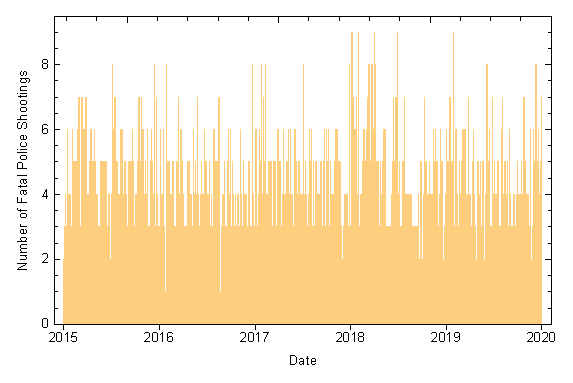
\includegraphics[height=7cm,width=14cm]{Overall(2).eps}
	\caption{Number of fatal police shootings each day from Jan. 1, 2015 to Dec. 31, 2019.}
	\end{figure}

	We notice that there are five days with 9 fatal police shootings recorded and four of them happened in 2018.

\section{Goodness-of-fit test for Poisson distribution}
	In \textit{London murders: a predictable pattern?}, David Spiegelhalter and Arthur Barnett assumed that “if murders happened as random events, the number of murders each day would follow a Poisson distribution” [1]. Similarily, we may assume that the fatal police shootings happened as random events, and the number of fatal police shootings would also follow a Poisson distribution. In order to confirm our assumption, we will test whether the occurrence of fatal police shootings in the USA follows a Poisson distribution or not from 2015 to 2019. From the data, we get the following table (Table 1).

\begin{table}[H]
\centering
\begin{spacing}{1.10}
\begin{tabular}{|c|c|c|c|c|c|c|c|c|c|c|}
\hline
\begin{tabular}[c]{@{}c@{}}Number of fatal police \\ shootings in a day\end{tabular} & 0   & 1   & 2   & 3   & 4   & 5   & 6  & 7  & 8  & 9 \\ \hline
Observed days                                                                    & 139 & 348 & 414 & 382 & 280 & 151 & 66 & 28 & 13 & 5 \\ \hline
\end{tabular}
\end{spacing}
\caption{Observed days with different numbers of fatal police shootings.}
\end{table}

	Let $X$ denotes the number of fatal police shootings in a day, then the maximum-likelihood estimator for $k$ is the sample mean [4], 
\begin{equation}
\begin{split}
\hat{k}=\bar{X}&= \frac{1}{5\cdot365+1} (139\cdot0+348\cdot1+414\cdot2+382\cdot3+ \\  & \quad \   280\cdot4+151\cdot5+66\cdot6+28\cdot7+13\cdot8+5\cdot9) \\
&=2.7043.
\nonumber
\end{split}
\end{equation}

	Then, in order to use the multinomial distribution, we should calculate 
\begin{equation}
\begin{split}
&P[X=0]=\frac{e^{-\hat{k}}{\hat{k}}^0}{0!}=0.0669; \qquad \qquad \qquad P[X=1]=\frac{e^{-\hat{k}}{\hat{k}}^1}{1!}=0.1810;  \\
&P[X=2]=\frac{e^{-\hat{k}}{\hat{k}}^2}{2!}=0.2447; \qquad \qquad \qquad P[X=3]=\frac{e^{-\hat{k}}{\hat{k}}^3}{3!}=0.2206;  \\
&P[X=4]=\frac{e^{-\hat{k}}{\hat{k}}^4}{4!}=0.1491; \qquad \qquad \qquad P[X=5]=\frac{e^{-\hat{k}}{\hat{k}}^5}{5!}=0.0807;  \\
&P[X=6]=\frac{e^{-\hat{k}}{\hat{k}}^6}{6!}=0.0364; \qquad \qquad \qquad P[X=7]=\frac{e^{-\hat{k}}{\hat{k}}^7}{7!}=0.0140;  \\
&P[X=8]=\frac{e^{-\hat{k}}{\hat{k}}^8}{8!}=0.0047;\\
&P[X\ge9]=1-P[X=0]-P[X=1]-\cdots-P[X=8]=0.0019.
\nonumber
\end{split}
\end{equation}

	Therefore, the distribution of $X$ can be expressed as a new distribution with a categorical random variable with parameters $(p_0,\,p_1,\,\cdots,\,p_9)=(0.0669,\, 0.1810,\,\cdots,\,0.0019)$.

	After that, we need to calculate the expected days with $E_i=np_i$, where $i$ is the category and $n$ is the sample size $n=5\cdot365+1=1826$.
\begin{equation}
\begin{split}
&E_0=1826\cdot0.0669=122.19; \qquad \qquad \qquad E_1=1826\cdot0.1810=330.45;  \\
&E_2=1826\cdot0.2447=446.81; \qquad \qquad \qquad E_3=1826\cdot0.2206=402.76;  \\
&E_4=1826\cdot0.1491=272.30; \qquad \qquad \qquad E_5=1826\cdot0.0807=147.27;  \\
&E_6=1826\cdot0.0364=66.38; \qquad \qquad \qquad \,\, \, E_7=1826\cdot0.0140=25.64;  \\
&E_8=1826\cdot0.0047=8.67; \qquad \qquad \qquad\,\, \,\,\, \, E_9=1826\cdot0.0019=3.47.
\nonumber
\end{split}
\end{equation}

	Besides, we should pay attention to the Cochran's Rule, which requires that
\begin{equation}
\begin{split}
&E[X_i]=np_i\ge1\qquad \qquad {\rm for\ all}\ i=1,\,\cdots,\,k,\\
&E[X_i]=np_i\ge5\qquad \qquad {\rm for\ 80\% \ of\ all}\ i=1,\,\cdots,\,k.
\nonumber
\end{split}
\end{equation}

	We find that all of the $E_i$s are greater than 1 and only one out of ten that is smaller than 5, which mean 90\% of the $E_i$s are greater than 5. Therefore, it satisfies the Cochran's Rule, and we can create the following table (Table 2).

\begin{table}[H]
\centering
\begin{spacing}{1.10}
\setlength{\tabcolsep}{1.5mm}{
\begin{tabular}{|c|c|c|c|c|c|c|c|c|c|c|}
\hline
\begin{tabular}[c]{@{}c@{}}Number of fatal police \\ shootings in a day\end{tabular} & 0      & 1      & 2      & 3      & 4      & 5      & 6     & 7     & 8    & 9    \\ \hline
Expected days                                                                        & 122.19 & 330.45 & 446.81 & 402.76 & 272.30 & 147.27 & 66.38 & 25.64 & 8.67 & 3.47 \\ \hline
Obseved days                                                                         & 139    & 348    & 414    & 382    & 280    & 151    & 66    & 28    & 13   & 5    \\ \hline
\end{tabular}}
\end{spacing}
\caption{Expected and observed days with different numbers of fatal police shootings.}
\end{table}

\begin{figure}[H]
\centering
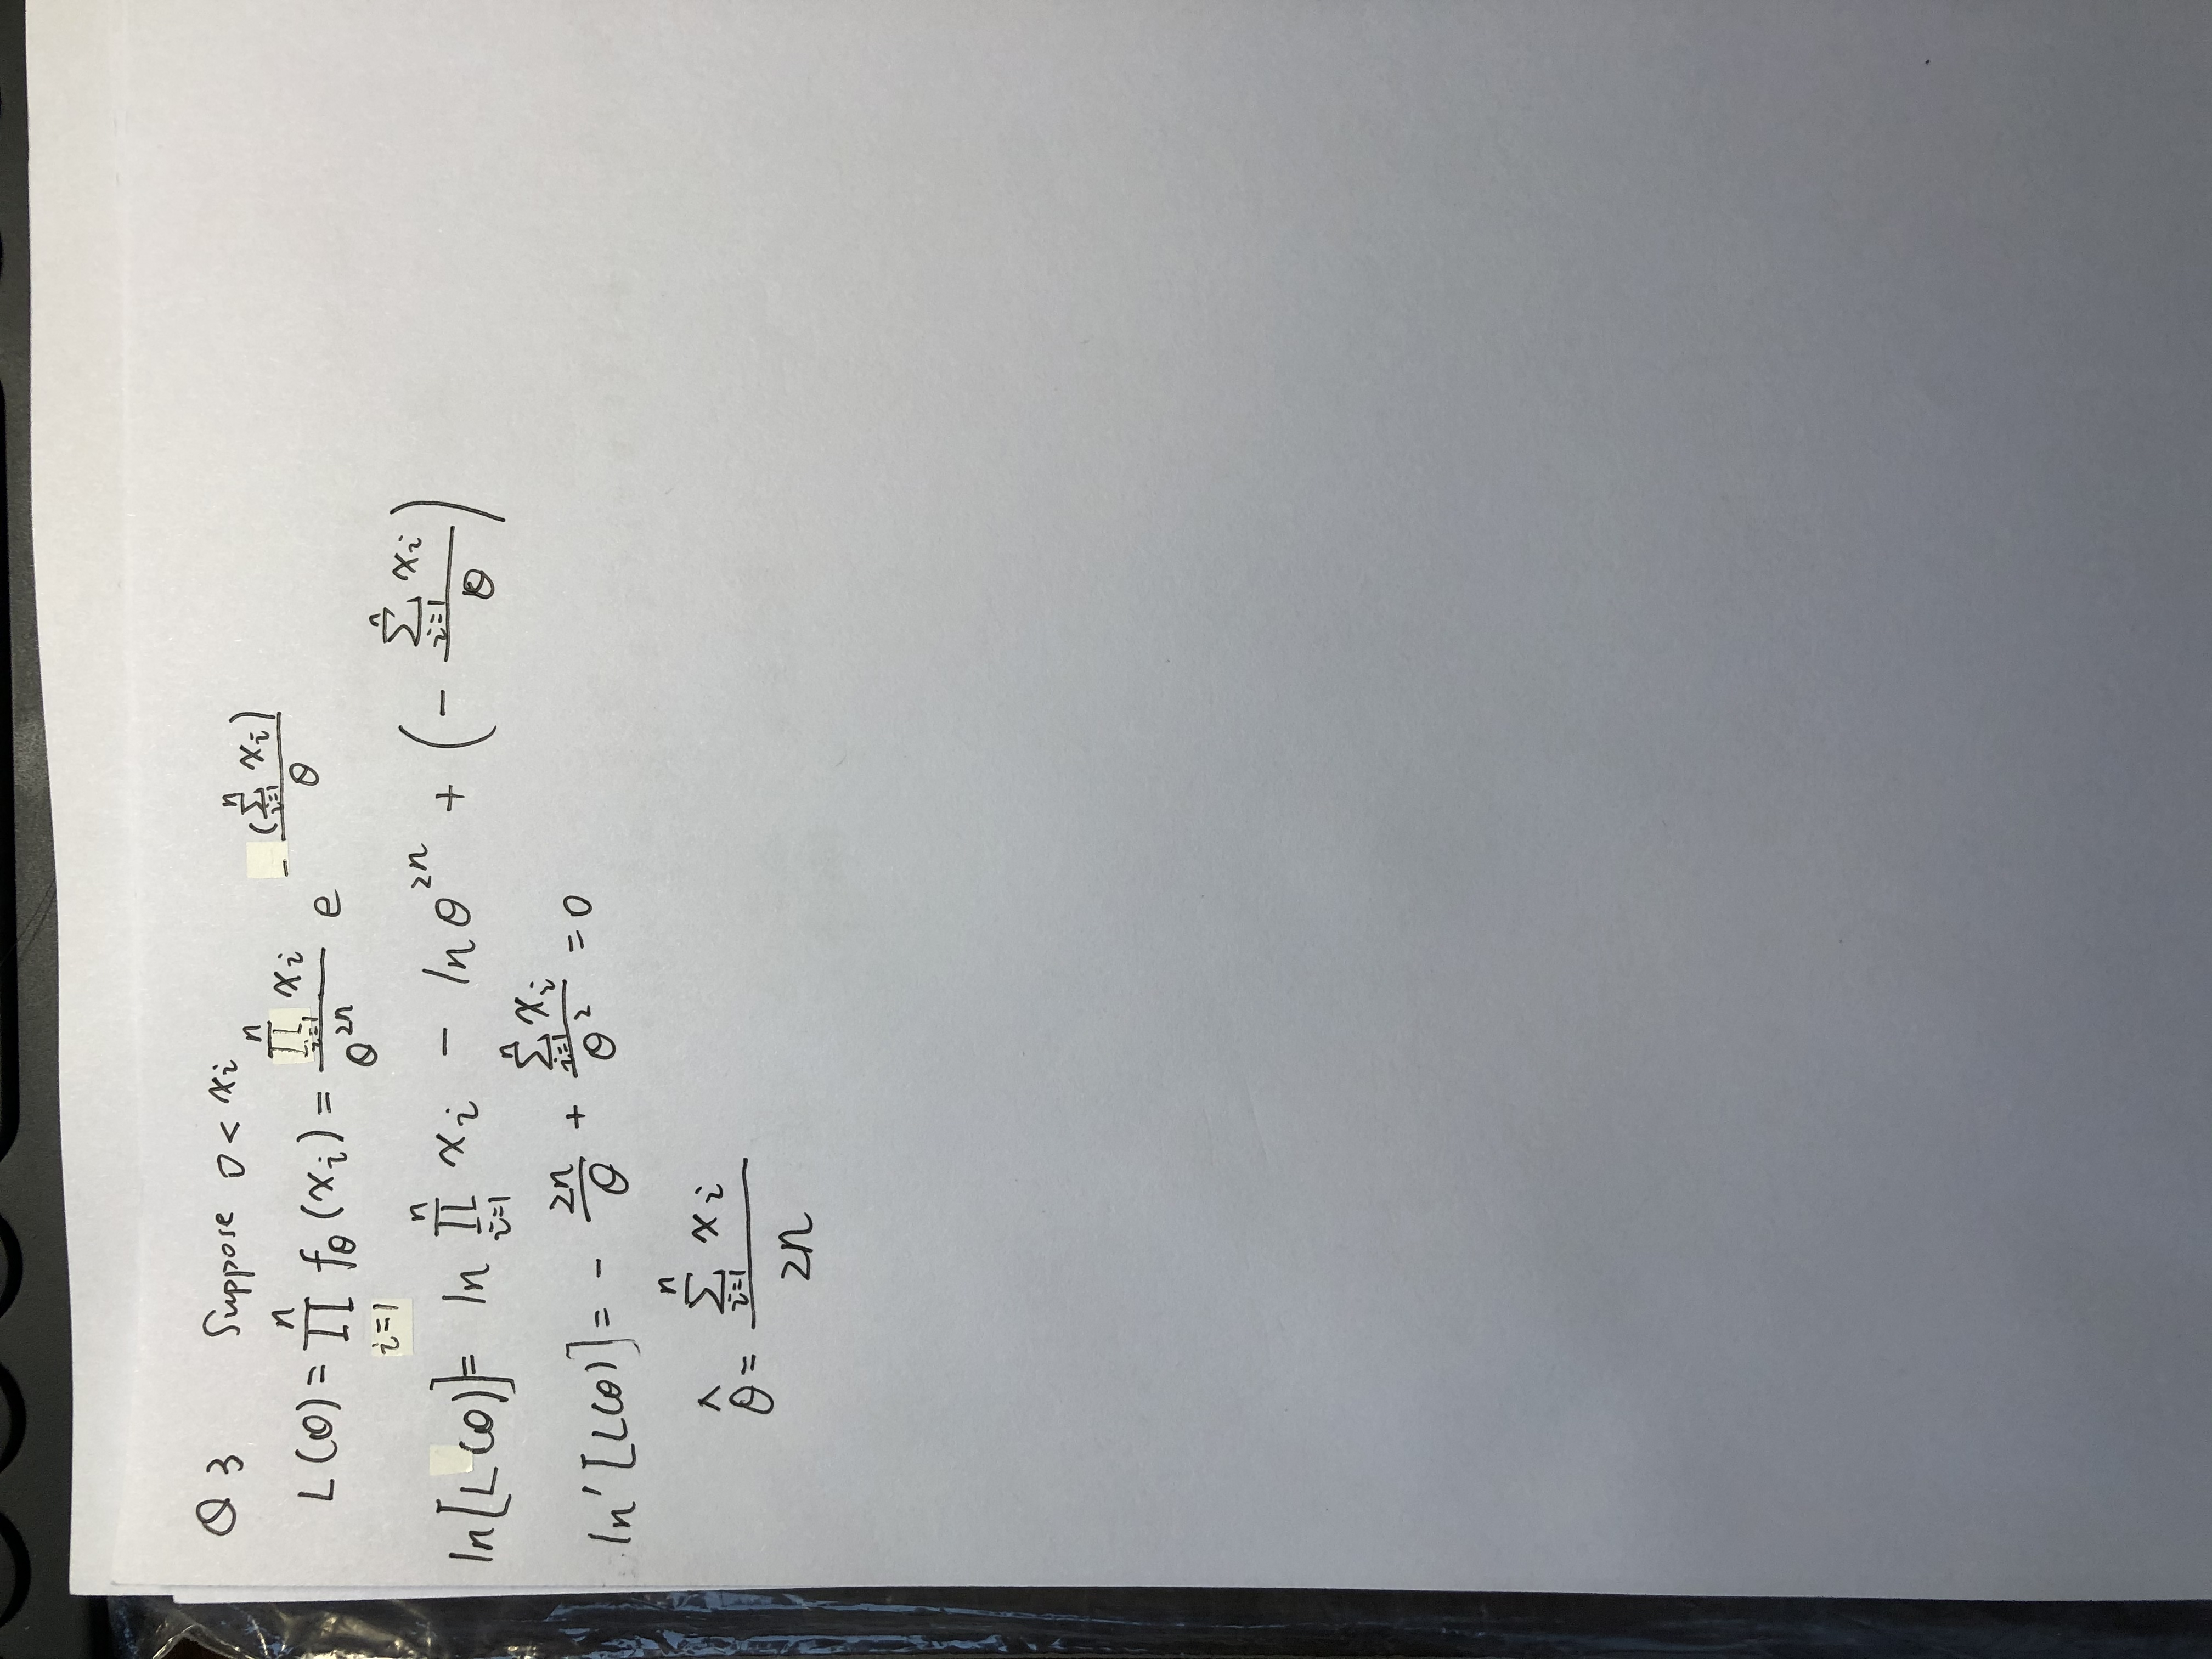
\includegraphics[height=5cm,width=15cm]{3.eps}
\captionsetup{justification=centering}
\caption{Days with different numbers of fatal police shootings: (a) expected; (b) observed.}
\end{figure}

	Then, the hypothesis “$H_0$: the number of fatal police shootings follows a Poisson distribution with parameter $k=2.7043$” is equivalent to “$H_0$: the number of fatal police shootings follows a multinomial distribution with parameters $(0.0669,\, 0.1810,\,\cdots,\,0.0019)$”. Besides, $$X^2=\sum_{i=1}^N\frac{(O_i-E_i)^2}{E_i}$$ follows a chi-squared distribution with $N-1-m=10-1-1=8$ degree of freedom, where $O_i$ is the observed value and $m$ is the number of parameters that we estimate. After we plug in the number, we get $X^2=10.94$. Let $\alpha=0.05$, we have $\chi_{0.05,\,8}^2=15.51\ge10.94$. Therefore, we are unable to reject $H_0$ at the 5\% level of significance. We can calculate the $P$-value as follows $$P=P[X^2|H_0]\le P[\chi_8^2\ge10.94]=1-P[\chi_8^2\le10.94]=1-0.7949=0.2051.$$The $P$-value is quite large, therefore, we cannot reject $H_0$, and we should consider that the number of fatal police shootings during Jan. 1, 2015 and Dec. 31, 2019 follows a Poisson distribution with parameter $k=2.7043$ [5].

\section{Dependence on weekday}
	From the data, we can also create the following figures that shows the number of fatal police shootings on each weekday and month (Figure 3).
\begin{figure}[H]
\centering
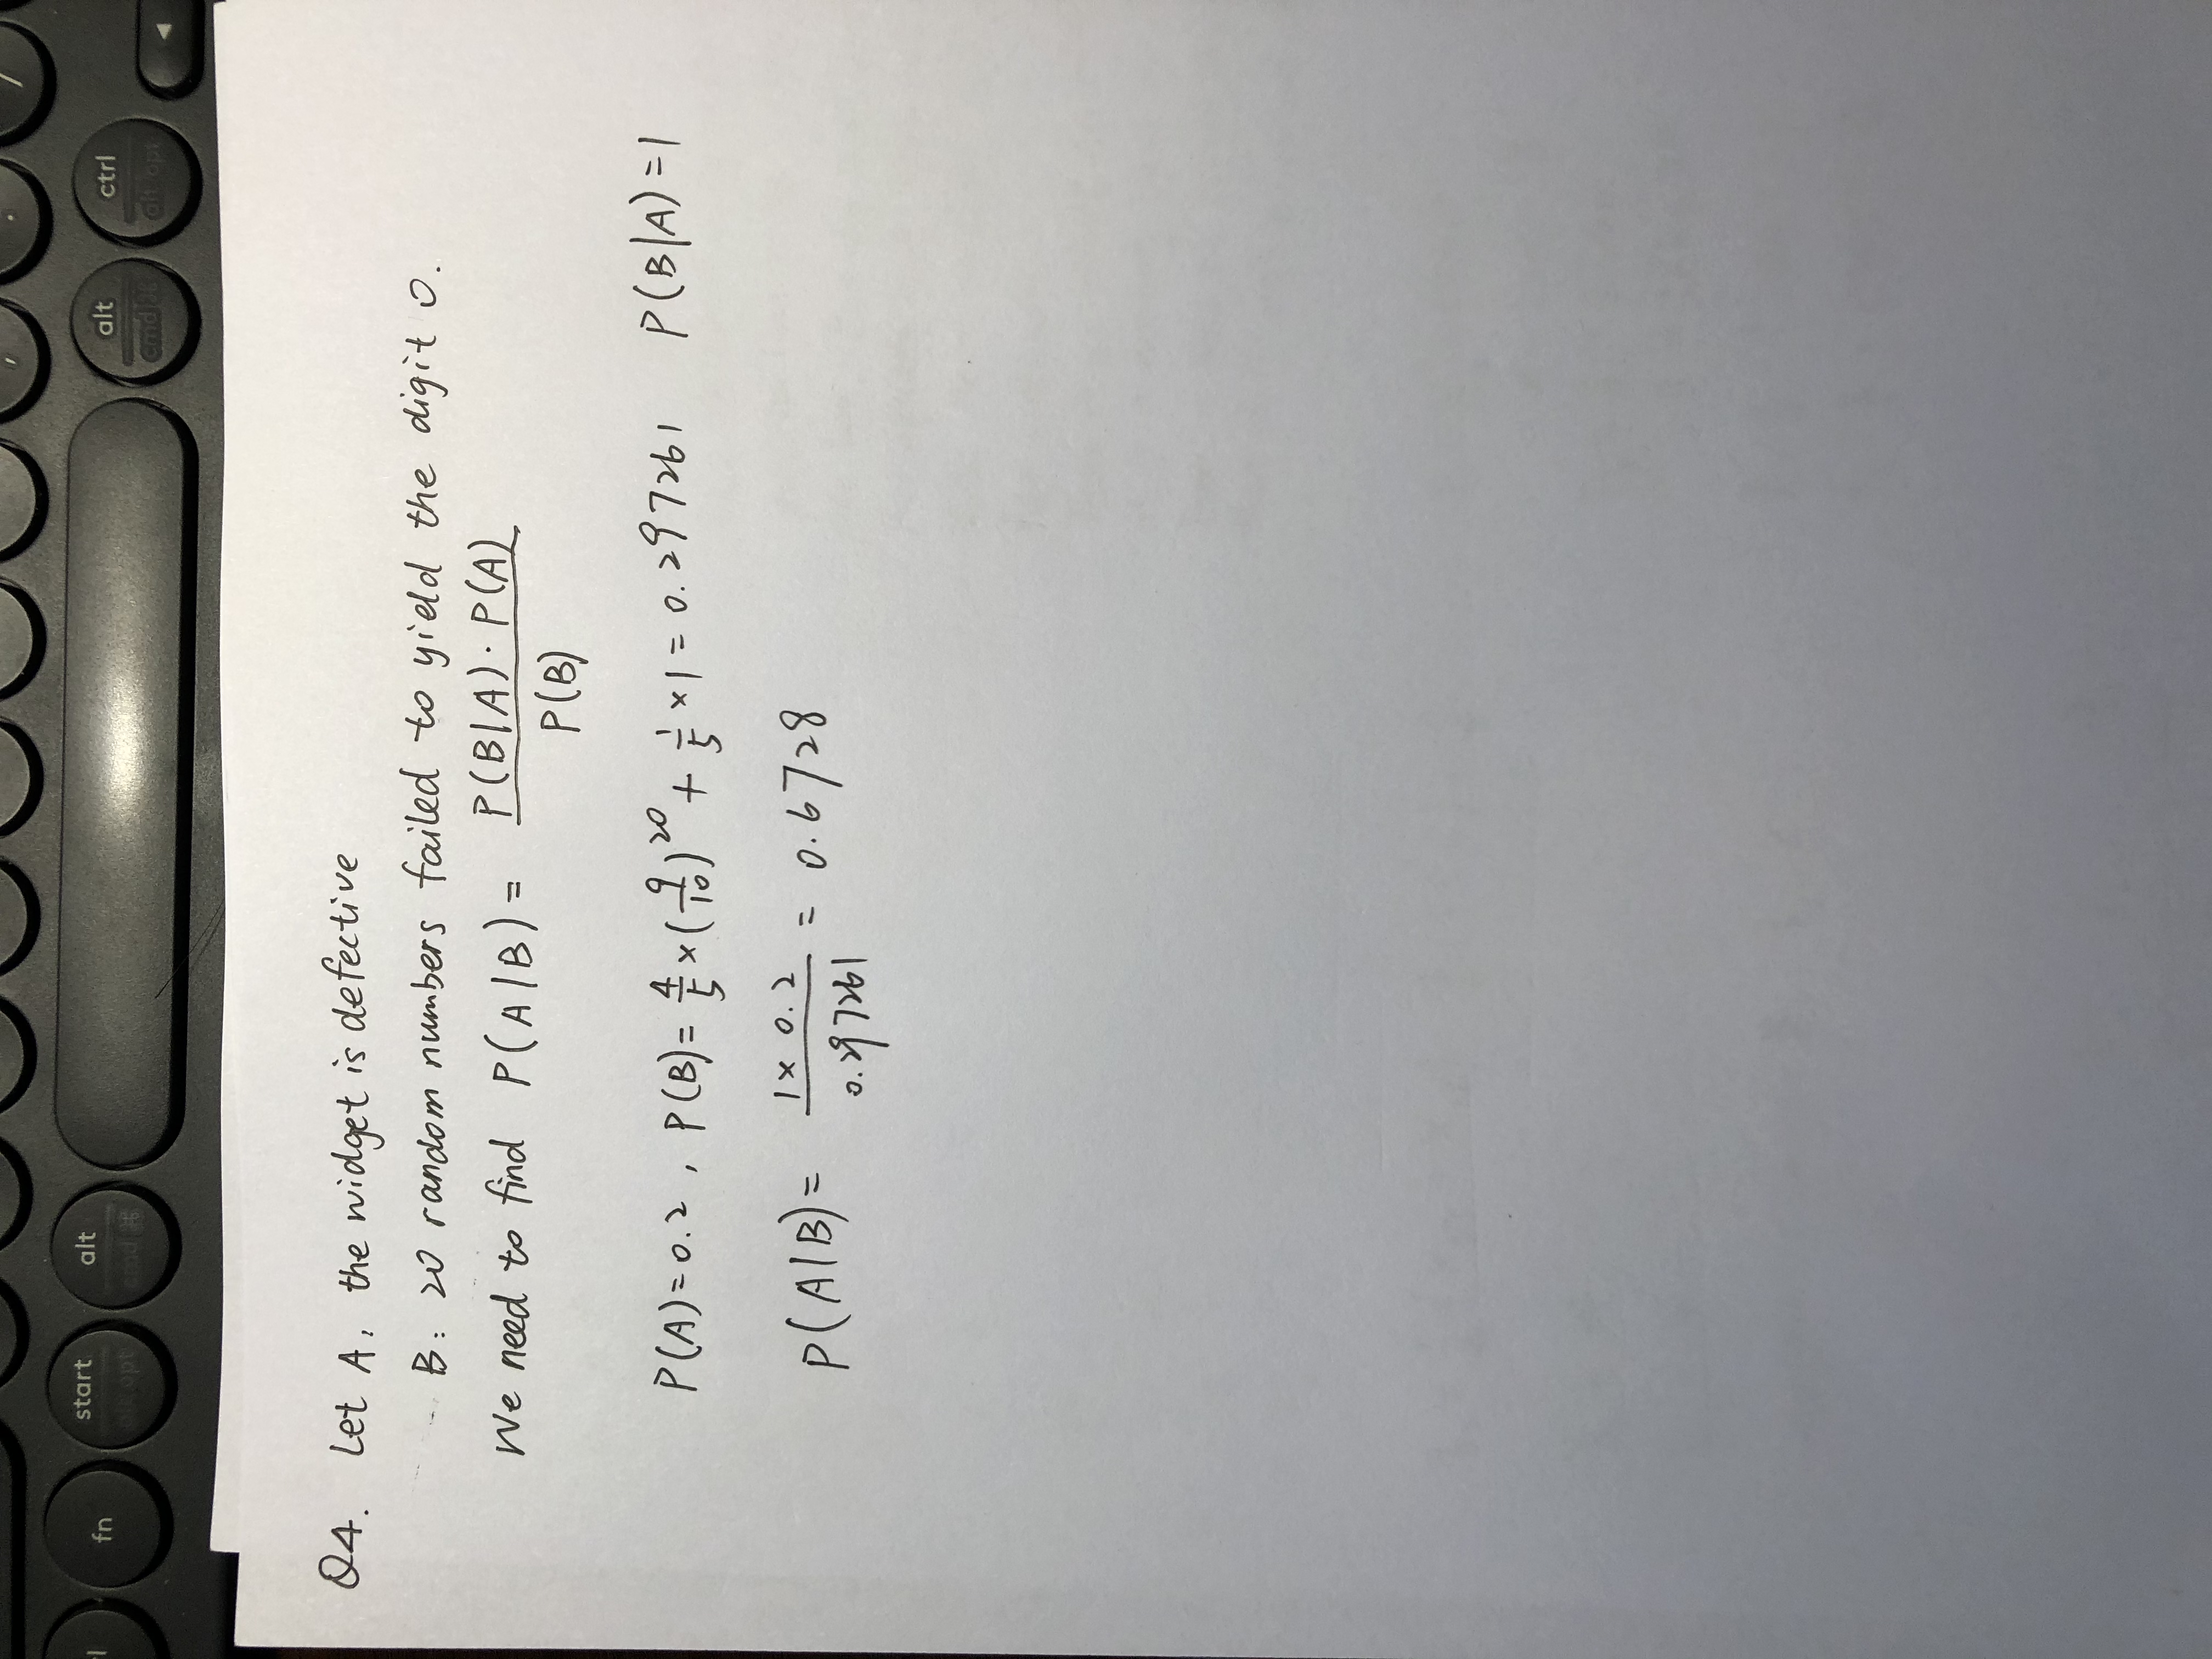
\includegraphics[height=4.5cm,width=13.5cm]{4.eps}
\captionsetup{justification=centering}
\caption{Number of occurrence of police shootings on (a) different weekdays and (b) different months.}
\end{figure}

We want to test whether there is evidence that the average number of police shootings depends on the weekday, then we should set the null hypothesis as “$H_0$: the number of fatal police shootings follows a multinomial distribution with the same parameter $p=\frac{1}{7}$” because there are seven different weekdays. There are 4938 fatal police shootings in total, so we can calculate the expected value on each weekday:
$$E_i=np_i=4938\times\frac{1}{7}=705.43.$$
Then we can get the following table (Table 3).
\begin{table}[H]
\centering
\begin{spacing}{1.10}
\begin{tabular}{|c|c|c|c|c|c|c|c|}
\hline
Weekdays         & Mon.   & Tue.   & Wed.   & Thu.  & Fri.   & Sat.   & Sun.   \\ \hline
Expected numbers & 705.43 & 705.43 & 705.43 & 705.43 & 705.43 & 705.43 & 705.43 \\ \hline
Obseved numbers  & 668    & 742    & 757    & 732    & 692    & 662    & 685    \\ \hline
\end{tabular}
\end{spacing}
\caption{Expected and observed number of fatal police shootings on diferent weekdays.}
\end{table}

We notice that it satisfies the Cochran's Rule because all the $E_i$s are greater than 5. Therfore,
$$X^2=\sum_{i=1}^7\frac{(O_i-E_i)^2}{E_i}=\frac{(668-705.43)^2}{705.43}+\cdots+\frac{(685-705.43)^2}{705.43}=12.17$$ follows a chi-square distribution with $N-1-m=7-1-0=6$ degree of freedom. Let $\alpha=0.05$, we have $\chi_{0.05,\,6}^2=12.59\ge12.17$. Therefore, we fail to reject $H_0$ at the 5\% level of significance, which means we can consider that the occurrence of fatal police shootings is independent on weekdays.

\section{Confidence interval for the parameter k of the Poisson distribution}

	We know that for a Poisson distribution, we have $E[X]=k$ and $Var[X]=k$ and we've already proved that $\bar{X}$ is an unbiased estimator for the parameter $k$ [4]. In our case we have a large sample size, so we can assume that $\bar{X}$ approximately follows a normal distribution with mean $k$ and variance $S/\sqrt{n}$. Then,
	$$\frac{\hat{k}-k}{S/\sqrt{n}}$$
is apprixomately standard-normally distributed.

	It follows that the $100(1-\alpha)\%$ confidence interval for k is given as follow [6]:
	
	$$\hat{k}\pm z_{\alpha/2}S/\sqrt{n}$$
	
	Furthermore, we note that $S^2$ is also an unbiased estimator for $k$ [4]. Thus we can substitute $S$ with $\sqrt{\hat{k}}$ and rewrite the $100(1-\alpha)\%$ confidence interval:
	
	$$\hat{k}\pm z_{\alpha/2}\sqrt{\hat{k}/n}$$
	
	Based on the data from 2015 to 2018, we have 4938 fatal police shooting in the total 1461 days [2]. Thus we have:
	
	\begin{equation}
	\hat{k}=\bar{X}=\frac{3934}{1461}=2.69.
	\end{equation}

	We use 95\% confidence interval as an example:
	
	$$\hat{k}\pm z_{\alpha/2}\sqrt{\hat{k}/n}=2.69\pm1.96\times\sqrt{2.69/1461}=2.69\pm0.084$$
	
\section{Goodness-of-fit test for data for 2020}

    To check whether the data for 2020 so far follows a Poisson distribution, we will apply the goodness-of-fit test. We first use the unbiased estimator $\bar{X}$ to estimate the parameter $k$.
    Based on the available data [2], we have:
    \begin{equation}
    \hat{k}_{2020}=\bar{X}=\frac{303}{106}=2.86.
    \end{equation}
    
    Then we can calculate the expected probability and the corresponding frequency of the Poisson distribution, which is calculated as follow and recorded in Table 4. 
    
\begin{equation}
\begin{split}
&P[X=0]=\frac{e^{-\hat{k}}{\hat{k}}^0}{0!}=0.057; \qquad \qquad \qquad P[X=1]=\frac{e^{-\hat{k}}{\hat{k}}^1}{1!}=0.164;  \\
&P[X=2]=\frac{e^{-\hat{k}}{\hat{k}}^2}{2!}=0.234; \qquad \qquad \qquad P[X=3]=\frac{e^{-\hat{k}}{\hat{k}}^3}{3!}=0.223;  \\
&P[X=4]=\frac{e^{-\hat{k}}{\hat{k}}^4}{4!}=0.160; \qquad \qquad \qquad P[X=5]=\frac{e^{-\hat{k}}{\hat{k}}^5}{5!}=0.091;  \\
&P[X=6]=\frac{e^{-\hat{k}}{\hat{k}}^6}{6!}=0.044; \qquad \qquad \qquad P[X=7]=\frac{e^{-\hat{k}}{\hat{k}}^7}{7!}=0.018;  \\
&P[X\ge8]=1-P[X=0]-P[X=1]-\cdots-P[X=7]=0.009.
\nonumber
\end{split}
\end{equation}
    
\begin{equation}
\begin{split}
&E_0=106\cdot0.057=6.1; \qquad \qquad \qquad E_1=106\cdot0.164=17.4;  \\
&E_2=106\cdot0.234=24.8; \qquad \qquad \qquad E_3=106\cdot0.223=23.7;  \\
&E_4=106\cdot0.160=16.9; \qquad \qquad \qquad E_5=106\cdot0.091=9.7;  \\
&E_6=106\cdot0.044=4.6; \qquad \qquad \qquad \,\, \, E_7=106\cdot0.018=1.9;  \\
&E_8=106\cdot0.009=0.9; \qquad \qquad \qquad\,\, \,\,\, \, 
\nonumber
\end{split}
\end{equation}    
    
    \begin{table}[H]
    \centering
    \begin{tabular}{|c|c|c|c|c|c|c|c|c|c|}
    \hline
    &0&1&2&3&4&5&6&7&8 or more\\
    \hline
    Probability&0.057&0.164&0.234&0.223&0.160&0.091&0.044&0.018&0.009\\
    \hline
    Expected Numbers&6.1&17.4&24.8&23.7&16.9&9.7&4.6&1.9&0.9\\
    \hline
    
    \end{tabular}
    \caption{Probability and expected frequency of days with different numbers of fatal police shooting in the US.}
    \end{table}
    
	Besides, we should pay attention to the Cochran's Rule, which requires that
\begin{equation}
\begin{split}
&E[X_i]=np_i\ge1\qquad \qquad {\rm for\ all}\ i=1,\,\cdots,\,k,\\
&E[X_i]=np_i\ge5\qquad \qquad {\rm for\ 80\% \ of\ all}\ i=1,\,\cdots,\,k.
\nonumber
\end{split}
\end{equation}    
    
    Thus we combine the last three categories together and carry out the null hypothesis that
    
    \begin{center}
    $H_0$: The data for 2020 so far follows a Poisson distribution with parameter $k=2.86$.
    \end{center}
    
    We compare the observed data with the expected data to decide whether to reject the null hypothesis or not. The pattern is recorded in Table 5 and Figure 4.
    
    \begin{table}[H]
    \centering
    \begin{tabular}{cccccccc}
    \hline
    \multicolumn{8}{c}{Numbers of days with the following numbers of fatal police shooting per day:}\\
    \hline
    \hline
    &0&1&2&3&4&5&6 or more\\
    \hline
    Expected&6.1&17.4&24.8&23.7&16.9&9.7&7.4\\
    \hline
    Observed&7&18&27&18&14&13&9\\
	\hline
    \end{tabular}
    \caption{Expected and observed number of days with 0, 1, 2 etc. fatal police shooting in the US on 105 days between January $1^{st}$ 2020 and April $15^{th}$ 2020.}
    \end{table}
    
    \begin{figure}[H]
    \centering
    \subfigure[]{
	\begin{minipage}[t]{0.47\linewidth}
	\centering
	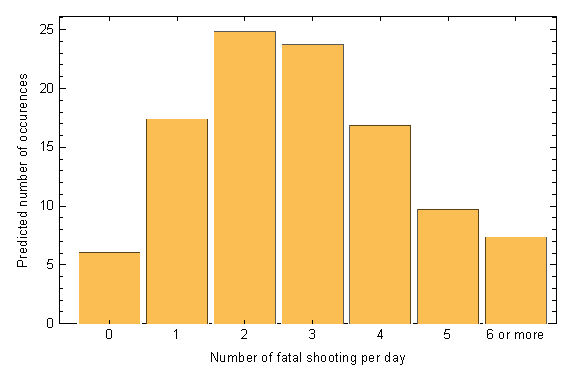
\includegraphics[width=69mm,height=45mm]{data_expected_14.eps}
	\end{minipage}
	}
	\subfigure[]{
	\begin{minipage}[t]{0.47\linewidth}
	\centering
	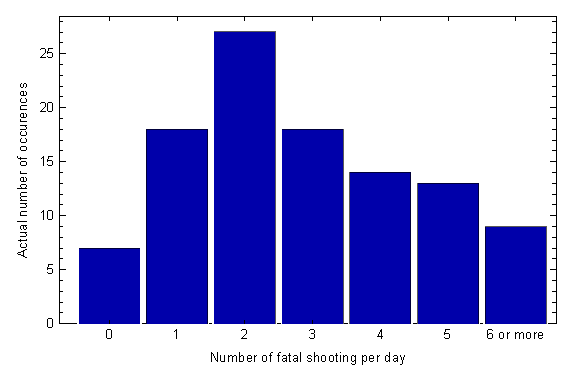
\includegraphics[width=69mm,height=45mm]{data_observed_14.eps}
	\end{minipage}
	}
	\caption{Frequency of occurance of days with different numbers of fatal police shooting recorded in the US between January $1^{st}$ 2020 and April $15^{th}$ 2020: (a) expected; (b) observed.}
    \end{figure}
    
    From the above data and bar charts, we can find that the observed data doesn't fit with the expected one. We will apply the $\chi^2$ test to the data to give a quantitative result.
    
    For $N=7$ categories, the statistic
    
    $$X^2=\sum\limits_{i=1}^N\frac{(O_i-E_i)^2}{E_i}$$
    then follows a chi-distribution with $N-1-m=7-1-1=5$ degrees of freedom.
    
    \begin{align*}
    X^2&=\frac{(7-6.1)^2}{6.1}+\frac{(18-17.4)^2}{17.4}+\frac{(27-24.8)^2}{24.8}+\frac{(18-23.7)^2}{23.7}+\frac{(14-16.9)^2}{16.9}+\frac{(13-9.7)^2}{9.7}+\frac{(9-7.4)^2}{7.4}\\
    &=3.68
    \end{align*}
    
	On the other hand, the critical value for $\alpha=0.05$ is $\chi^2_{0.05,5}=11.1$. Since $X^2<\chi^2_{0.05,5}$, we have no evidence to reject the null hypothesis that the data for 2020 so far follows a Poisson distribution with $k=2.86$.
	
	The result shows that the data for 2020 follows a Poisson distribution, which corresponds to our expectation. However, we also find that the pattern doesn't fit with the expected one very well. From Figure 4 we can find that the number of 3 shooting per day is relatively fewer than expected [5].

\section{Prediction interval for 2020}
	According to the article “Improved closed-form prediction intervals for binomial and Poisson distributions”, we can use the Nelson prediction interval to predict the future counts of a Poisson distribution [7].
	
	We will first define some parameters used in calculation: let $\lambda$ be the mean of the Poisson distribution; in the sample size of $n$, there are a total of $X$ existing arrivals;in another sample size of $m$, there will be a total of $Y$ future arrivals [7].
	
	First it is easy to find that the estimator $\hat{\lambda}=\bar{X}=\frac{X}{n}$. At the same time, $\hat{\lambda}=\frac{\hat{Y}}{m}$. According to these two equations, we have:
	
	\begin{equation}
	\hat{\lambda}=\frac{X}{n}
	\hat{Y}=\frac{mX}{n}
	\end{equation}

Also to estimate the variance of $m\hat{\lambda}-Y$, we calculate as follow:

\begin{align*}
\hat{Var}(m\hat{\lambda}-Y)&=\hat{Var}(\frac{mX}{n}-Y)\\
&=\frac{m^2}{n^2}\hat{Var}(x)+\hat{Var}(Y)\\
&=\frac{m^2}{n^2}n\hat{\lambda}+m\hat{\lambda}\\
&=m^2\lambda(\frac{1}{n}+\frac{1}{m})
\end{align*}

Thus we have:

\begin{equation}
\hat{Var}(m\hat{\lambda}-Y)=m^2\hat{\lambda}(\frac{1}{n}+\frac{1}{m})
\end{equation}

Then we need to verify that

$$\frac{m\hat{\lambda}-Y}{\sqrt{\hat{Var}(m\hat{\lambda-Y})}}$$
is standard-normally distributed, which is equal to verifying that $m\hat{\lambda}-Y$ has mean 0. We've already proved that $\hat{\lambda}=X/n$ and $\hat{Y}=mX/n$. Therefore, the formula above follows a standard normal distribution [7].

According to the article, the Nelson prediction interval is given by $[\lceil L \rceil,\lfloor U\rfloor]$ [7]. Thus instead of conducting the two-sided test, we need to conduct two one-sided respectively. We calculate $\lceil L\rceil$ as an example.

Since $\frac{m\hat{\lambda}-Y}{\sqrt{\hat{Var}(m\hat{\lambda}-Y)}}$ follows a standard normal distribution, we have 
\begin{align*}
\alpha&=P\bigg[\frac{m\hat{\lambda}-Y}{\sqrt{\hat{Var}(m\hat{\lambda}-Y)}}\leqslant z_{1-\alpha}\bigg]\\
&=P\bigg[m\hat{\lambda}-z_{1-\alpha}\sqrt{\hat{Var}(m\hat{\lambda}-Y)}\leqslant Y\bigg]\\
&=P\bigg[\hat{Y}-z_{1-\alpha}\sqrt{m\hat{Y}\bigg(\frac{1}{n}+\frac{1}{m}\bigg)}\bigg]
\end{align*}

Similarly, we can calculate the upper bound and thus we can get

\begin{equation}
[L,U]=\hat{Y}\pm z_{1-\alpha}\sqrt{m\hat{Y}\bigg(\frac{1}{m}+\frac{1}{n}\bigg)}
\end{equation}

	From the above formula, we can derive a 95\% prediction interval for 2020 based on the data for 2015 to 2019 [2]. In this case, the parameters are listed as follow:
	
	\begin{table}[H]
	\centering
	\begin{tabular}{cc}
	$X=4938$&$n=1826$\\
	$\alpha=0.05$&$z_{1-\alpha}=1.645$\\
	\end{tabular}
	\end{table}
	
	Then we can use the data to obtain the prediction interval:
	
	$$\frac{mX}{n}\pm z_{1-\alpha}\sqrt{\frac{m^2X}{n}\bigg(\frac{1}{m}+\frac{1}{n}\bigg)}=\frac{4938m}{1826}\pm1.645\times\sqrt{\frac{4938m^2}{1826}\bigg(\frac{1}{m}+\frac{1}{1826}\bigg)}$$
	
	After simplification, we obtain the 95\% prediction interval shown by the following formula:
	
	\begin{equation}
	2.704m\pm1.645\sqrt{2.704m+0.0015m^2}
	\end{equation}

	Figure 5 shows the predicted number of fatal police shooting in the US during 2020 (the black solid line) and the 95\% prediction limits (the dash lines) with the data for 2020 so far (the red dots).
	
	\begin{figure}[H]
    \centering
    \subfigure[Predicted number of fatal police shooting in the US during 2020(with 95\% prediction limits)]{
	\begin{minipage}[t]{0.47\linewidth}
	\centering
	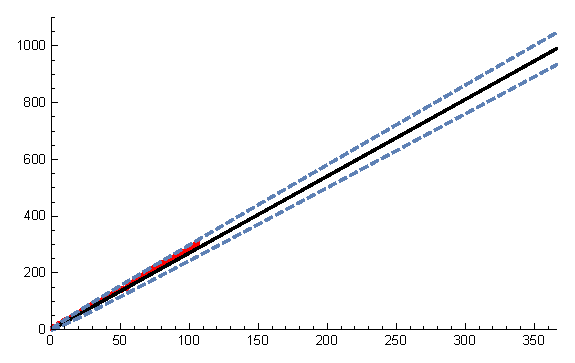
\includegraphics[width=69mm,height=45mm]{prediction_over.eps}
	\end{minipage}
	}
	\subfigure[Predicted number of fatal police shooting in the US during 2020(with 95\% prediction limits) and the data for 2020 so far in detail]{
	\begin{minipage}[t]{0.47\linewidth}
	\centering
	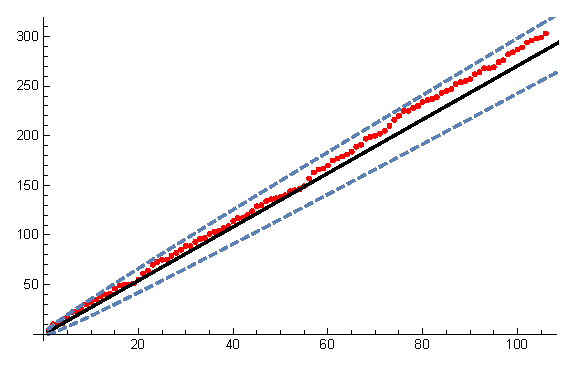
\includegraphics[width=69mm,height=45mm]{prediction_detail.eps}
	\end{minipage}
	}
	\caption{Predicted number of fatal police shooting in the US during 2020 with 95\% prediction limits: (a) overview; (b) detailed.}
    \end{figure}
    
    From Figure 5, we can find that the data for 2020 lies in the prediction interval quite well. This indicates that based on the data for 2015-2019, we can roughly predict the future tendency of the fatal police shooting.

\section{The influence of the outbreak of Coronavirus}

	We must note that the Poisson distribution model is based on the assumption that “the level of violence remains the same” [1]. However, when taking the outbreak of the Coronavirus into account, we should be careful whether this will influence our original assumption.
	
	Before focusing on the influence of the outbreak of COVID-19 on fatal police shooting, we may first have a general idea of the situation of COVID-19 in the US. The following figure (Figure 6) is a screenshot of the number of people confirmed COVID-19 in the US provided by Johns Hopkins University. The marked point is the data for March $27^{th}$, when the confirmed people first exceeds 100k people and reaches 101.7k people [8].
	
	\begin{figure}[H]
	\centering
	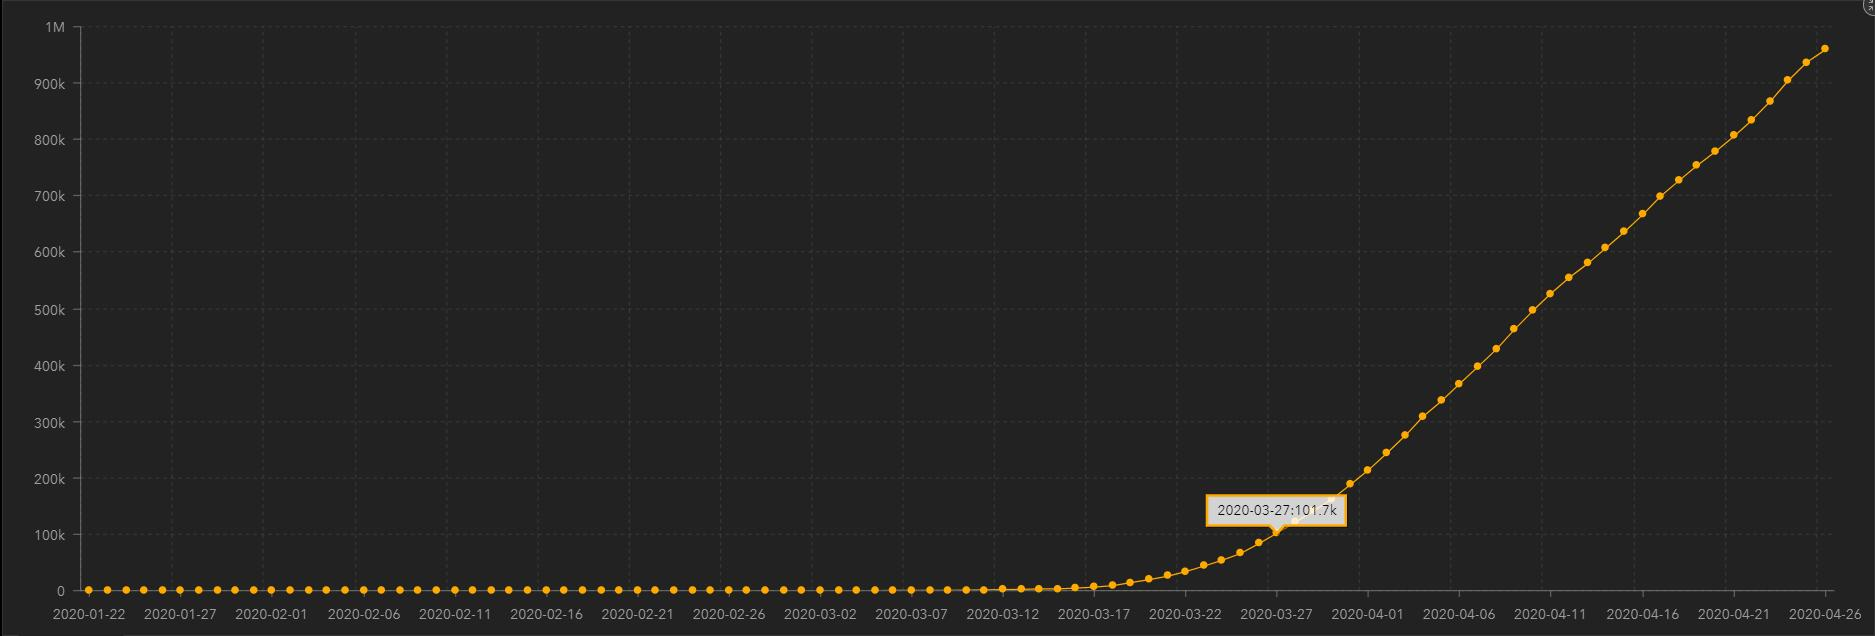
\includegraphics[width=122.2mm,height=42.3mm]{covid19.jpg}
	\caption{Number of people confirmed COVID-19 in the US [8].}
	\end{figure}
	
	If we look deep into the data, we can find that there's no strong evidence indicating that the outbreak of COVID-19 has a strong influence on the fatal police shooting generally since the previous sections have reached the conclusion that the data for 2020 still follows a Poisson distribution and the data so far all falls in the prediction interval.
	
	However, we may still get some information from the data. If we turn to Figure 5, we may find that for the first half of the data so far, it is really close to the exact predicted line. For the second half of the data, however, the number of fatal police shooting is rising relatively faster and is approaching the upper bound of the prediction interval. The turning point is in March, which is also the time when COVID-19 broke out in the US.
	
	The reason why the number is rising may be due to the following several reasons:
	
	1. The outbreak of COVID-19 makes the residents penic and thus more people are likely to do extreme things.
	
	2. The US government doesn't respond to the epidemic properly and effectively, leading to some citizens' discontent to the government.

	3. Some recidents doesn't obey the government's control measures and have conflicts with the police.
	
\section{Conclusion}
	
	The project mainly analyze the data of fatal police shooting in the US for 2015-2019 and predict the possible tendency in 2020. We first specify the definition of “fatal” and give a general overview of the data. For the first half of the project, we mainly analyze the data for 2015-2019 by checking its fitness to the Poisson distribution, the confidence interval of the parameter $k$ of the Poisson distribution and the relationship between fatal police shooting and each weekday and month. In the second half of the project, we focus on the data for 2020. We test its fitness to the Poisson distribution based on the existing data for 2020 and also predict its future pattern. At last we take the outbreak of COVID-19 into account and analyze its influence on fatal police shooting.
	
	Through this project, we confirm that the data for fatal police shooting follows a Poisson distribution. Based on the previous data, we can also predict the future possible numbers of fatal police shooting to a certain extent. Moreover, considering the special situation this year, namely the outbreak of COVID-19, it's still not quite clear whether it will significantly influence fatal police shooting.


\section{Reference}
[1] D. Spiegelhalter and A. Barnett, “\textit{London murders: a predictable pattern?}” Significance, vol. 6, no. 1, pp. 5–8, 2009. \url{http://onlinelibrary.wiley.com/doi/10.1111/j.1740-9713.2009.00334.x/abstract}.

[2] The Washington Post, “\textit{Data-police-shootings},” GitHub. \url{https://github.com/washingtonpost/data-police-shootings}. Accessed April 28, 2020.

[3] The Washington Post, “\textit{Fatal force}.” \url{https://www.washingtonpost.com/graphics/national/police-shootings-2016/}. Accessed April 19, 2020.

[4] H. Hohberger, “\textit{Ve401\_video\_12},” UMJI-SJTU, pp. 18-19, 2020.

[5] H. Hohberger, “\textit{Ve401\_video\_23},” UMJI-SJTU, pp. 9-36, 2020.

[6] H. Hohberger, “\textit{Ve401\_video\_13},” UMJI-SJTU, pp. 8-9, 2020.

[7] K. Krishnamoorthy and Jie Peng, “\textit{Improved closed-form prediction intervals for binomial and Poisson distributions}” Journal of Statistical Planning and Inference, vol. 141, no.5, pp. 1709-1718, 2011. \url{http://www.sciencedirect.com/science/article/pii/S0378375810005215}.

[8] Johns Hopkins University. Coronavirus Resource Center. “\textit{COVID-19 United States Cases by County}.” \url{https://coronavirus.jhu.edu/us-map}. Accessed April 28, 2020.

\newpage

\section{Appendix}
	\subsection{Code for 3.2 Overview of the data}
\begin{lstlisting}
data := Import["shootingdata.csv"][[2 ;; 4939, 3]]
DateHistogram[data, "Day", 
 Ticks -> {{"2015", "2016", "2017", "2018", "2019", "2020"}, 
   Automatic}, Frame -> True, 
 FrameLabel -> {"Date", "Number of Fatal Police Shootings"}]
\end{lstlisting}
\

	\subsection{Code for 4 Goodness-of-fit test for Poisson distribution}
\begin{lstlisting}
BarChart[{122.19, 330.45, 446.81, 402.76, 272.30, 147.27, 66.38, 
  25.64, 8.67, 3.47}, 
 ChartLabels -> {"0", "1", "2", "3", "4", "5,", "6", "7", "8", 
   "9 or more"}, Frame -> True, 
 FrameLabel -> {"Number of fatal police shootings per day", 
   "Predicted number of occurrences"}, PlotRange -> {0, 450}]

BarChart[{139, 348, 414, 382, 280, 151, 66, 28, 13, 5}, 
 ChartLabels -> {"0", "1", "2", "3", "4", "5,", "6", "7", "8", 
   "9 or more"}, Frame -> True, 
 FrameLabel -> {"Number of fatal police shootings per day", 
   "Actual number of occurrences"}, PlotRange -> {0, 450}, 
 ChartStyle -> Darker[Blue]]
\end{lstlisting}
\

	\subsection{Code for 5 Dependence on weekday}
\begin{lstlisting}
data := Import["shootingdata.csv"][[2 ;; 4939, 3]]
DateHistogram[data, "Day", DateReduction -> "Week", Frame -> True, 
 FrameLabel -> {None, "Number of Fatal Police Shootings"}]
DateHistogram[data, "Month", DateReduction -> "Year", Frame -> True, 
 FrameLabel -> {None, "Number of Fatal Police Shootings"}]
\end{lstlisting}

	\subsection{Code for 7 Goodness-of-fit test for data for 2020}
\begin{lstlisting}
BarChart[{6.1, 17.4, 24.8, 23.7, 16.9, 9.7, 7.4}, 
 ChartLabels -> {"0", "1", "2", "3", "4", "5", "6 or more"}, 
 Frame -> True, 
 FrameLabel -> {"Number of fatal shooting per day", 
   "Predicted number of occurences"}]

BarChart[{7, 18, 27, 18, 14, 13, 9}, 
 ChartLabels -> {"0", "1", "2", "3", "4", "5", "6 or more"}, 
 Frame -> True, 
 FrameLabel -> {"Number of fatal shooting per day", 
   "Actual number of occurences"}, ChartStyle -> Darker[Blue]]
\end{lstlisting}

	\subsection{Code for 8 Confidence interval for the parameter k of the Poisson distribution}

\begin{lstlisting}
Show[ListPlot[
  {4, 10, 10, 11, 17, 22, 23, 25, 30, 32,
   35, 38, 40, 41, 46, 49, 50, 50, 51, 55,
   61, 64, 70, 73, 75, 75, 79, 82, 85, 89, 89,
   93, 96, 97, 101, 103, 104, 107, 109, 114, 117,
   117, 120, 124, 129, 130, 134, 136, 137, 138, 140,
   144, 145, 146, 149, 157, 163, 166, 167, 170,
   175, 177, 179, 181, 184, 189, 191, 197, 199, 200,
   202, 205, 210, 216, 220, 225, 225, 228, 230, 234,
   236, 237, 239, 243, 245, 247, 252, 254, 255, 257, 262,
   264, 268, 268, 269, 274, 276, 282, 284, 287, 289,
   294, 296, 298, 299, 303}, PlotStyle -> Red, 
  PlotRange -> {{0, 366}, {0, 1100}}, PlotStyle -> SmallCircle], 
 Plot[2.704*m, {m, 1, 366}, PlotStyle -> Black, Frame -> Ture, 
  PlotRange -> {{0, 366}, {0, 1100}}], 
 Plot[2.704*m + 1.645*Sqrt[2.704*m + 0.0015*m^2], {m, 1, 366}, 
  PlotStyle -> Dashed, PlotRange -> {{0, 366}, {0, 1100}}], 
 Plot[2.704*m - 1.645*Sqrt[2.704*m + 0.0015*m^2], {m, 1, 366}, 
  PlotStyle -> Dashed, PlotRange -> {{0, 366}, {0, 1100}}]]
  
  Show[ListPlot[
  {4, 10, 10, 11, 17, 22, 23, 25, 30, 32,
   35, 38, 40, 41, 46, 49, 50, 50, 51, 55,
   61, 64, 70, 73, 75, 75, 79, 82, 85, 89, 89,
   93, 96, 97, 101, 103, 104, 107, 109, 114, 117,
   117, 120, 124, 129, 130, 134, 136, 137, 138, 140,
   144, 145, 146, 149, 157, 163, 166, 167, 170,
   175, 177, 179, 181, 184, 189, 191, 197, 199, 200,
   202, 205, 210, 216, 220, 225, 225, 228, 230, 234,
   236, 237, 239, 243, 245, 247, 252, 254, 255, 257, 262,
   264, 268, 268, 269, 274, 276, 282, 284, 287, 289,
   294, 296, 298, 299, 303}, PlotStyle -> Red, 
  PlotStyle -> SmallCircle], 
 Plot[2.704*m, {m, 1, 366}, PlotStyle -> Black, Frame -> Ture], 
 Plot[2.704*m + 1.645*Sqrt[2.704*m + 0.0015*m^2], {m, 1, 366}, 
  PlotStyle -> Dashed], 
 Plot[2.704*m - 1.645*Sqrt[2.704*m + 0.0015*m^2], {m, 1, 366}, 
  PlotStyle -> Dashed]]
\end{lstlisting}

\end {document}